% Node-link MLP diagram in pure TikZ (Neutelings-style, self-contained).
% Compile: pdflatex mlp_tikz.tex
\documentclass[border=8pt]{standalone}
\usepackage{tikz}
\usetikzlibrary{arrows.meta}

\colorlet{colin}{blue!60!black}
\colorlet{colhid}{green!45!black}
\colorlet{colout}{red!60!black}

\tikzset{
  >=Latex,
  neuron in/.style={circle, draw=colin,  fill=blue!18,  minimum size=0.72cm, inner sep=0},
  neuron hid/.style={circle, draw=colhid, fill=green!18, minimum size=0.72cm, inner sep=0},
  neuron out/.style={circle, draw=colout, fill=red!18,   minimum size=0.72cm, inner sep=0},
  link/.style={-{Latex[length=1.5mm]}, gray!55, thin},
}

\begin{document}
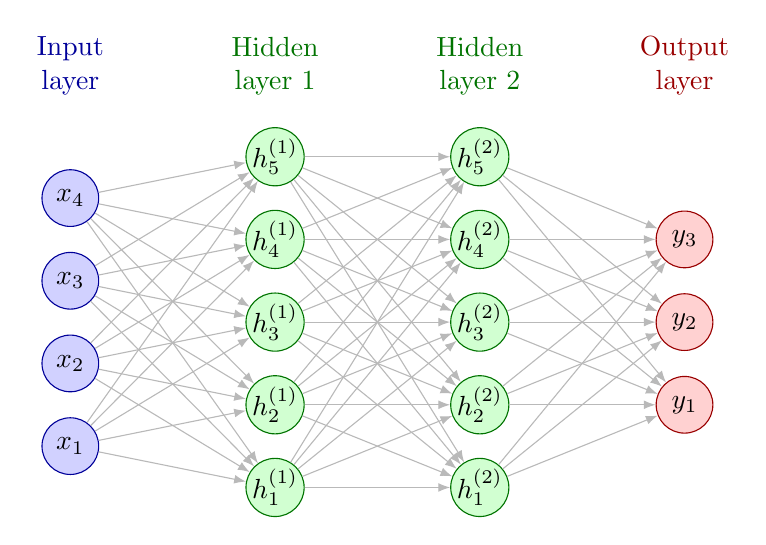
\begin{tikzpicture}[x=2.6cm, y=1.05cm]

  % ---- neurons: one \foreach per layer, vertically centred
  \foreach \i in {1,...,4}
    \node[neuron in]  (I\i) at (0, {\i - 2.5}) {$x_{\i}$};
  \foreach \i in {1,...,5}
    \node[neuron hid] (H\i) at (1, {\i - 3.0}) {$h^{(1)}_{\i}$};
  \foreach \i in {1,...,5}
    \node[neuron hid] (G\i) at (2, {\i - 3.0}) {$h^{(2)}_{\i}$};
  \foreach \i in {1,...,3}
    \node[neuron out] (O\i) at (3, {\i - 2.0}) {$y_{\i}$};

  % ---- fully-connected links: nested \foreach per layer pair
  \foreach \i in {1,...,4} \foreach \j in {1,...,5}
    \draw[link] (I\i) -- (H\j);
  \foreach \i in {1,...,5} \foreach \j in {1,...,5}
    \draw[link] (H\i) -- (G\j);
  \foreach \i in {1,...,5} \foreach \j in {1,...,3}
    \draw[link] (G\i) -- (O\j);

  % ---- layer captions
  \node[colin,  align=center] at (0, 3.1) {Input\\layer};
  \node[colhid, align=center] at (1, 3.1) {Hidden\\layer 1};
  \node[colhid, align=center] at (2, 3.1) {Hidden\\layer 2};
  \node[colout, align=center] at (3, 3.1) {Output\\layer};

\end{tikzpicture}
\end{document}
